\documentclass[10pt,twocolumn]{article}

\usepackage{url}
\usepackage{ulem}\normalem
\usepackage{graphicx}
\usepackage{lettrine}
\usepackage{multicol}
\usepackage{verbatim}
\usepackage{subfigure}
\usepackage[usenames,dvipsnames,table]{xcolor}
\usepackage[ruled,vlined,linesnumbered]{algorithm2e}


\usepackage{boxedminipage}

\newcommand{\commentary}[2]{{\bf {\sc #1:} \emph{#2}}}
\newcommand{\guillaume}[1]{\commentary{guillaume}{#1}}
\newcommand{\hector}[1]{\commentary{hector}{#1}}
\newcommand{\corina}[1]{\commentary{corina}{#1}}


\clubpenalty=10000
\widowpenalty=10000

\renewcommand{\topfraction}{0.9}	% max fraction of floats at top
\renewcommand{\textfraction}{0.1}
\renewcommand{\floatpagefraction}{0.8}
\setcounter{topnumber}{1}

% the fixme command
\newcommand{\fixme}[1]
{
  \noindent
  \begin{boxedminipage}{\linewidth}
    \textsl{{\bf FIXME: #1}}
  \end{boxedminipage}
}

\begin{document}

\begin{multicols}{2}
\title{Robust Performance Control for Web Applications in the Cloud}
\author{Hector Fernandez, Corina Stratan, Guillaume Pierre, Eliana Tirsa and Valentin Cristea} 
\date{Vrije Universiteit Amsterdam and University Politehnica of Bucharest}
\maketitle
\end{multicols}


%\section{Introduction}
% Magazine articles have no section called "Introduction"

Talk about wikipedia outage, traffic spikes and amazon outages "Popular websites crippled by hours-long Amazon cloud service outage"

Talk about vertical and horizontal scaling
Measuring instance performance
Multi instance infrastrucutres

Even if we use two level threshold there are traffic oscillations which cannot be handled by the system due to minimal variations. These minimal oscillations can sometimes be higher than the own infrastructure cost and degradate the user experience. In this paper, we try to minimize these by using a heterogonouer resource provisioning system. the cost of the infrastructure

Contribution:
App metrics instead of other system which hare limited to VM-level metrics. (Pluggable autoscaling service)
Real application and traces
Cost considerations.
Decision making scaling up/down out/in.
Dynamic load balancing
Measuring instance performance without additional resources

SLO fulfillment in order to avoid the cost of slo penalties.
Type of machines
SLO penalty -- different type of customers

Explain what is a scaling plan

\section*{ConPaaS overview \label{conpaas}}

Make an overview of the base ConPaaS system, without details on  
provisioning.

\begin{itemize}
\item the ConPaaS manager and agents
\item Ganglia integration
\item the provisioning / profiling manager
\end{itemize}

Possibly make a diagram with all these components.

\section*{The Wikipedia application \label{wikipedia}}

%To evaluate the behavior and accuracy of ConPaaS when hosting web applications, we prepared a realistic and complex enough scenario to assess any PaaS. In particular, we deployed the Wikipedia web application called MediaWiki~\cite{mediawiki}, and used a web hosting benchmark called WikiBench~\cite{wikibench}. 

%1. The heterogenity of the requests of wikipedia and realistic scenario.

Most academic resource provisioning systems are evaluated using
synthetic applications and workloads such as TPC-W, RuBiS and
RuBBoS. However, these traditional benchmarks do not exhibit features
of real Web applications such as traffic unstability as well as
heterogeneous and constantly-changing request mixes~\cite{benchlab}.
Instead of basing our evaluations on unrealistic workloads, we used
the WikiBench benchmark~\cite{wikibench}. This benchmark uses a full
copy of Wikipedia as the web application, and replays a fraction of
the actual Wikipedia's access traces.


%Wikipedia uses
%MediaWiki~\cite{mediawiki}, a PHP-based wiki software package.
%The architecture of the Wikipedia website uses a http-proxy, a http-web server, a database and one or more PhP servers. 
Hosting a copy of Wikipedia in ConPaaS requires two different
services: a PHP web hosting and a MySQL service. The MySQL service is
loaded with a full copy of the English Wikipedia articles as of 2008,
which has a size of approximately 30GB.  In the PHP service, the
configuration was composed of one load balancer, one static web server
and one or more PHP servers. We then use WikiBench to replay access
traces from 2008~\cite{urdaneta2009}.



%ConPaaS uses nginx as static web server and also as load balancer.% The PHP requests are handled through PHP FastCGI Process Manager.
%In the PhP service, an initial configuration was composed of one Nginx http-proxy, one Apache server, and one or more PhP (FastCGI Process Manager) servers. Each PhP server hosts the MediaWiki application which is the main component of this system. 

% 3. Presentation of the preeliminary experiment

%To evaluate our system we used Wikibench, a tool for
%benchmarking Wikipedia servers developed by our group. Wikibench
%replays Wikipedia access traces or smaller samples of the traces,
%providing various sampling mechanisms.
%We used anonymized Wikipedia access traces, which are published by the WikiMedia foundation, and for our experiments we replayed a sample of 10\% from the traces. 
The trace contains requests for static and dynamic pages. When
replaying it, the most important performance bottleneck is the
application logic of the application: PHP requests are processed an
order of magnitude slower than simpler static web pages. In this
article we therefore focus on the automatic scaling of the PHP tier.

As an example, in Figure~\ref{workload}, we show the PHP workload
sampled from one trace, as the number of PHP requests per minute
during approximately one day. Besides the obvious variations in number
of requess per minute, requests are also heterogeneous in complexity.
To illustrate this heterogeneity, in
Figure~\ref{phpRespTimeDispersion} we present the distribution of the
response time values for the PHP requests during the execution of the
trace shown in Figure~\ref{workload}.  For this experiment we used a
fixed number of 5 PHP servers, which are sufficient for handling the
workload from the access trace even at its peaks; this is why in this
case the response time is not influenced by the intensity of the
workload.  However, the results show a relatively wide dispersion of
the response time: the response time values of dynamic pages are
commonly spread over a factor 3 between the slowest and the fastest
requests.  The main reason for this dispersion is that the Wikipedia
articles vary in complexity, requiring different amounts of
information that needs to be retrieved from the database and assembled
in a page.

% 4. Expectations for the evaluation presented

We also conclude from this experiment that, since the response time of
the application varies and cannot be properly predicted even when the
request rate is known, a provisioning algorithm aiming to keep the
application's response time under a certain limit should take into
account several monitoring parameters beyond the request rate and the
response time.



%Similarly, as depicted by Figure~\ref{workload} and Figure~\ref{phpRespTimeDispersion}, there is not any correlation between the PhP request volumes and their response times. More precisely in Figure~\ref{phpRespTimeDispersion}, the highest response time values obtained in the interval of time 600min. match up with a drop in the request rate during the same interval in Figure~\ref{workload}. Therefore, any provisioning technique that makes decisions based on the request rate can incur errors by under- or over-provisioning an application, which can reduces the efficiency of the scaling actions. 


%I got the expected behavior different response time values independently of the req rate at each time. }

%\fixme{ OTHER POSSIBILITY: More precisely in Figure~\ref{reqRate}, the highest response time values obtained during the trace execution, %match up with low levels of requests rate. Therefore, ...  }

% Similarly, the intensity of the resulting traffic could also be modified ranging from very low up to the 
% original traffic intensity of the trace. 

%Initial benchmark results show a typical day of Wikipedia traffic and the relation between the request rate %and the server response times. 


\begin{figure}
\begin{center}
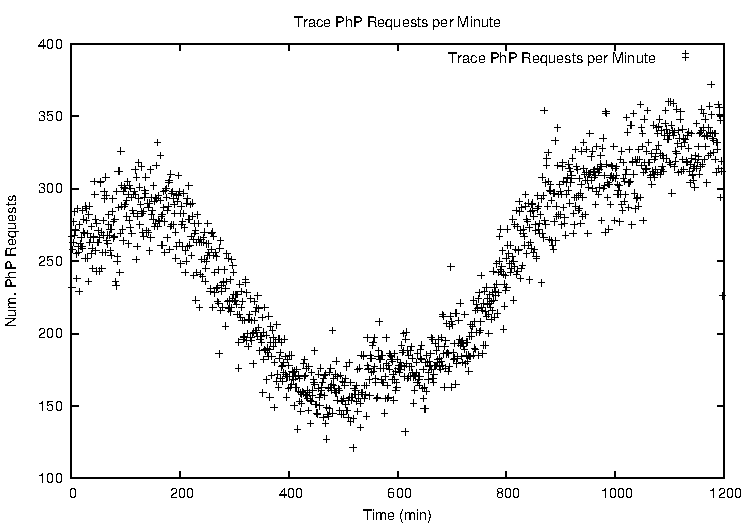
\includegraphics[width=0.49\textwidth, height=6cm]{./images/traceWorkload}
\end{center}
\vspace{-5mm}
\caption{Wikipedia trace workload.}
\label{workload}
\end{figure}

% Corina - I think this paragraph would be better suitable for future work:
%In addition, other properties may be also considered important when using the Wikipedia traces such as the interarrival time between requests, the distribution of page popularity, the mix of static/dynamic requests, the ratio of read/write operations and requests for non-existing pages and files.

%\begin{itemize}
%\item The intervarrival time between requests follows a Poisson distribution.

%\item The distribution of page popularity varies from very popular pages to those being accessed very infrequently.

%\item The mix of static/dynamic requests presents a strong variation. 

\begin{figure}
\begin{center}
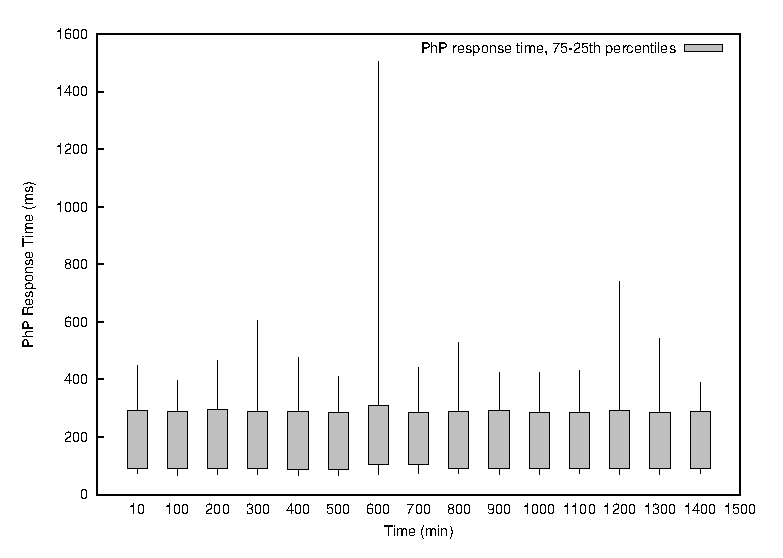
\includegraphics[width=0.49\textwidth, height=6cm]{./images/phpRespTimeDispersion}
\end{center}
\vspace{-5mm}
\caption{Complexity of PhP requests.}
\label{phpRespTimeDispersion}
\end{figure}

%\item The ratio of read/write operations vary having more reads than editions or creations of wiki pages.

%\begin{figure}
%\begin{center}
%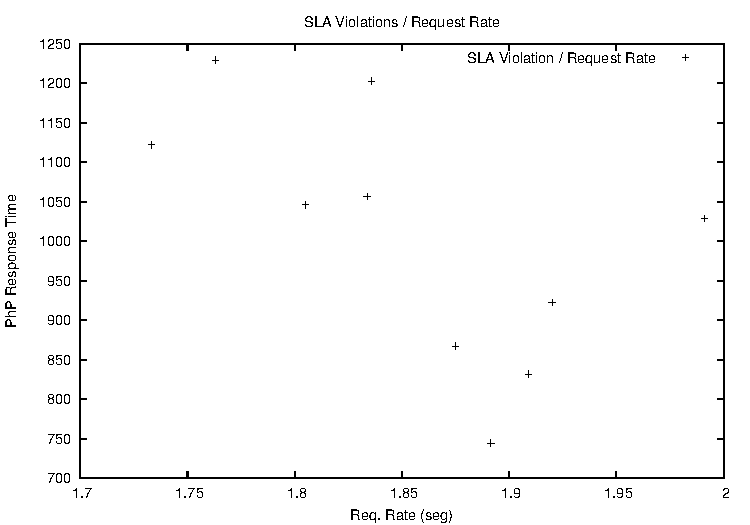
\includegraphics[width=0.49\textwidth, height=6cm]{./images/staticProv_reqRate}
%\end{center}
%\caption{Response time vs request rate.}
%\label{reqRate}
%\end{figure}

%\item A considerable amount of requests for non-existing pages and files add realism to the traffic.

%\end{itemize}


%By using real world server side software and data, we think the WikiBench benchmarking suite is a very  realistic and extensible research tool.

% these traces create workloads for WikiBench instead of creating purely synthetic workloads like other benchmarking tools have done.

%The workload-mix and the variable amount of data and visitors make of Wikipedia a valid example of elastic web application. In this paper, we focus in the scalability of the PhP web hosting service, and thereby as the number of PhP servers hosting MediaWiki scale out or back based on the demanding workload.



\section*{Resource provisioning \\algorithms \label{provisioning}}

We evaluated three resource provisioning algorithms: a trigger-based
algorithm representing a baseline comparable to systems currently in
production, and two new algorithms.


%\subsection{Load-based provisioning}
\subsection*{Trigger-based provisioning}

%\corina{I edited the following paragraphs to reflect the fact
%that Amazon and other clouds don't really provide the provisioning
%algorithms, they just provide means to implement them
%(i.e. the cloud users need to write the provisioning rules
%themselves). Also, I saw that now EC2 also provides support
%for the users to have custom monitoring metrics.}


%\hector{Yes, I agree I was thinking on rightscale ... good then.}

The existing cloud infrastructures provide means to implement
provisioning mechanisms that adjust the amount of allocated 
resources based on a number of standard monitoring parameters. 
These are simple trigger-based systems that define threshold 
rules to increase or decrease the amount of computational resources
when certain conditions are met. As an example, the Auto Scaling 
system offered by Amazon EC2~\cite{amazonEC2} can be used to define 
rules for scaling out or back an application based on monitoring
parameters like CPU utilization, network traffic volume etc. 
This trigger-based technique is currently used in well-known 
cloud platforms such as RightScale~\cite{right-scale} or OpenShift~\cite{openshift}. 

For the sake of comparison, we designed and implemented a
trigger-based provisioning mechanism in ConPaaS. This technique
monitors CPU usage and application response time metrics, and assigns
a lower and upper threshold for each metric. It then creates or
deletes VMs whenever one of the threshold is crossed. The thresholds
are statically defined by the user before execution.

\begin{algorithm} 
{\scriptsize
\SetAlgoLined
\SetInd{0mm}{2mm}
\KwData{ Pre-defined metric threshold ranges, \emph{SLO\_threshold}
}
\KwResult{Scaling decisions}
\BlankLine
\While{auto-scaling is ON}{
Collect monitoring data of each metric, \emph{data$_i$}\;
\BlankLine
\If{ no recent scaling operation}{
\uIf{ avg(data$_i$) $>=$ \emph{SLO\_threshold\_min}$_i$ for at least one metric }{
ADD resources\;
}
\ElseIf{ avg(data$_i$) $<$ \emph{SLO\_threshold\_max}$_i$ for all metrics }{
REMOVE resources\;
} 
%}\Else{ Sleep during 5minutes \;}
} 
Sleep for 5 minutes \; 
}
}
\caption{Trigger-based}
\label{triggerBased_prov}
\end{algorithm}

% , expressed in the form of a Service Level Agreement


%\subsubsection{Problematic of this algorithm}
%subsubsection{Drawbacks of this algorithm}

Even though this is simple and widely used in cloud platforms, we show
that it is too reactive because of the following reasons:

%regarding the decision making process
%\corina{I removed the item about services as black boxes, because now
%Amazon provides support for custom parameters; and also because we also
%implemented the trigger-based algorithm with custom parameters (request
%rate, response time) so our implementation doesn't see the service
%as a black-box either.}


\begin{itemize}
\item  \textbf{Workload heterogeneity:} For some web sites, the 
workload fluctuates following an irregular pattern, with occasional
short traffic spikes. An excessively reactive algorithm cannot handle
these situations well, and will cause frequent fluctuations in the number
of allocated resources; this has negative effects on the stability and
performance of the system, as well as increases the infrastructure cost. 

%Obviously, a reactive algorithm can be seen a good choice for resource provisioning, however. The system %performance of an application change in time if the type of workload changes.

%\item \textbf{Reactiveness:} An excessively reactive algorithm can affect 
%the system's stability, by causing frequent fluctuations in the number
%of allocated resources; this has negative effects on the performance, 
%as well as increases the infrastructure cost. 

%\item \textbf{Services as black boxes:} Services are handled as black boxes, the definition of threshold rules often only covers system-level metrics such as response time and CPU usage. Therefore, when provisioning web applications, metrics such as request rate of static/dynamic files may be also taken into consideration to improve the accuracy of the decisions.

% when handling web traffic.

%These constraints are too generic, as other application-specific constraints are not considered. 

%\item VMs are heterogeneous in performance, and thereby their throughput vary depending of its hardware configuration (instance's types). 
\item  \textbf{Resources heterogeneity:} The performance of virtual instances 
provided by current clouds is largely heterogeneous, even among
instances of the same type, as shown in~\cite{ec2Performance}.
Simple trigger-based provisioning systems do not take this heterogeneity
into account, thus providing less efficient resource allocation. 

% The provisioning mechanism omit the heterogeneity of the VMs associated to host an application. 

\end{itemize}

Based on these factors, we believe trigger-based provisioning mechanisms can 
be improved without drastically increasing their complexity. A possible 
solution is the utilization of techniques that handle workload and resource
heterogeneity without being excessively reactive. Moreover, the implementation 
of these techniques should remain simple to facilitate their integration in 
existing auto-scaling systems. In the following we present two techniques 
that aim at solving the aforementioned drawbacks by relying on predictive 
and more accurate methods.

% to dynamically adjust the computational power to irregular workload pattern of web applications.


%previous knowledge about behavior of the application, avoid flash crowds too reactive
%and the definition of application-specific constraints 
%Tthe definition of threshold range based on how much workload a server can handle. what is the request %rate that a server can sustain without becoming overloaded?
%what is the value of the CPU utilization/load that indicates that a server is
%overloaded? These values are different from one application to another, and also
%from one server to another. 


%Second experiment: improved the basic provisioning with some application knowledge
%observed empirically (the maximum request rate we can send to a server, maybe also
%the maximum CPU utilization we can allow). The results show more stability in the
%provisioning.  


\subsection*{Feedback provisioning}

%\corina{Generic suggestion about this section: I think we should give
%some better motivation/intuition about the 3 techniques presented
%in this section. Ideally it would have been to have separate experimental 
%results with each technique used just on its own, and see how much 
%improvement each technique brings. But since we don't have that,
%maybe you could just give some more explanations/intuition based
%on what you saw in the experiments, of why each technique works?}

%\hector{You mean to completely change the Section 3 and 4. I don't know if this will delay a lot the publication of this article. }

%Based on our previous knowledge from load-based provisioning, we designed and implemented an algorithm which improves the accuracy of our scaling actions %when hosting web applications. To achieve that, our algorithm relies on three simple mechanisms: the definition of weights to each metric included in the %performance requirements, the use of flexible thresholds and the estimation of the workload trend. 

To handle the workload heterogeneity and excessive reactiveness of trigger-based techniques, we designed and implemented an algorithm that relies on three simple mechanisms: the definition of weights to each metric included in the performance requirements, the estimation of the workload trend and the use of two-levels of threshold ranges. 

%In order to handle temporal bursty workload, we designed and implemented a predictive and reactive algorithm by relying on
\vspace{2mm}

%Traditional algorithms would scale out and back whenever a system-level metric exceeds its beforehand defined threshold range. 

\textbf{Weighted metrics:}  Through the definition of weight values to application and system metrics, our scaling decisions can adapt to the characteristics of the workload produced by an application. This mechanism allows to determine the weight of a metric based on its efficiency to rapidly alert of the existence of any degradation, as described in Algorithm~\ref{history_prov}. As such, to automatically obtain these weight values, this mechanims calculates the correlation coefficients associated to the response times in comparison with the metrics. As an example, when hosting the MediaWiki application, our algorithm associates to the CPU metric a higher weight than the request rate, since higher values in the CPU usage rapidly indicate the existence of a performance degradation, due to the large diversity in the complexity of the requests. As pointed out in~\cite{singh_autonomic_2010}, provisionins decisions solely made on the basis of request rate or CPU usage can incur errors  by under- or over-provisioning an application. This mechanism is also flexible, as users could define different sets of metric-weight pairs depending of the application.

% As pointed out in~\cite{singh_autonomic_2010} and \cite{roy_capacity_2011},

%algorithm takes into consideration its weight when making scaling decisions. This mechanism allows to define metric-weight pairs based on the expected type of %workload produced by an application, thus improving the accuracy of our decisions. Hence, the definition of weights determine the efficiency of a metric to rapidly %alert of the existence of any degradation before than others. Similarly, the set of metric-weight pairs could also be configured by the user, as it varies depending of %the application. As an example, when hosting the MediaWiki application, our algorithm associates weights in an ascending order to the following metrics: request %rate, CPU usage and response time. Accordingly the response time has a higher weight than the request rate, since higher values in the response time rapidly %indicate the existence of a performance degradation. 

%As detailed in Section~\ref{wikipedia}, scaling decisions only make based on the request rate can incur errors by under- or over-provisioning  a web application, %due to the large diversity in the complexity of the requests~\cite{singh_autonomic_2010}.

%High values in the request rate cannot always indicate that an application is becoming overloaded, due to the large diversity in the complexity of the requests.


\begin{algorithm}
{\scriptsize
\SetAlgoLined
\SetInd{0mm}{2mm}
\KwData{ Pre-defined metric threshold ranges, \emph{SLO\_threshold}
}
\KwResult{Scaling decisions}
\BlankLine
Create a queue to store historical workload, \emph{q}\;
Establish flexible thresholds: \emph{pred\_thr} and \emph{reac\_thr} \;
\BlankLine
\While{auto-scaling is ON}{
Collect monitoring data of each metric, \emph{data}\;
Calculate the weight of each metric, \emph{w}

\uIf{ avg(data$_i$) $>=$ pred\_thr\_max$_i$}{ \label{alg:thr1}
	Increment chances of \emph{scaling\_out}: \emph{s\_out} = \emph{s\_out} + \emph{w$_i$}\;
}\ElseIf{ avg(data$_i$) $<$ pred\_thr\_min$_i$}{
	Increment chances of \emph{scaling\_back}:  \emph{s\_bck} = \emph{s\_bck} + \emph{w$_i$}\; \label{alg:thr2}
\Else{
Decrease the chances: \emph{s\_bck} - \emph{w$_i$} or \emph{s\_out} - \emph{w$_i$}\;\label{alg:thr3}
}}
\BlankLine
Add to \emph{q} the most recent workload value\; \label{alg:esti1}
Estimate historical workload trends (last $\sim$30min), \emph{td}\;
\hspace{3mm}	- Increasing, \emph{td} = 1 / Decreasing, \emph{td} = 0\;	\label{alg:esti2}
\BlankLine
\If{ no recent scaling operation}{
\uIf{ avg(data$_i$) $>=$ reac\_thr\_max$_i$ \textbf{and}  $td$ = 1 \textbf{and} \emph{s\_out} $>$ \emph{s\_bck}}{ \label{alg:thr4}
	ADD resources\;
}
\ElseIf{ avg(data$_i$) $<$ reac\_thr\_min$_i$ \textbf{and} \emph{td} = 0 \textbf{and} s\_out $<$ s\_bck }{ \label{alg:thr5}
	REMOVE resources\;
}
Reset \emph{s\_bck} and\emph{s\_out}\;
}\Else{ Sleep during 5 minutes\;}
}
}
\caption{Feedback}
\label{history_prov}
\end{algorithm}

%\corina{I think here there should be explained better the usage and
%intuition behind s\_in and s\_out. They are used as extra conditions
%for scaling out and back, but I'm not sure I understand exactly when
%they play a role: if the response time exceeds the reactive threshold,
%in what situations can the extra condition with s\_in and s\_out prevent
%scaling out? Also, are s\_in and s\_out ever reset or decremented?}

\textbf{Workload's trend estimation:} Nowadays, there is a wide
literature on mathematical models that try to predict future
alterations in web application's workload. However, the workload
heterogeneity and network traffic of web applications make more
difficult to provide accurate predictions using these models. Besides,
the complexity of these models sometimes prevent its integration into
real auto scaling systems. To design a robust and simple provisioning
system, we decided to use a feedback mechanism that analyzes the
behavior of the system performance during a short interval of
time. Even though different intervals can be used, an analysis of the
monitoring data during approx. 30min (considering 15min between
scaling actions) provides enough information to detect the workload's
current trend, and thereby to classify the type of workload alteration
as \emph{constant} or \emph{temporal} (Algorithm~\ref{history_prov}
lines \ref{alg:esti1}-\ref{alg:esti2}). Only \emph{constant}
variations may trigger scaling actions to avoid frequent fluctuations
in the system performance caused by short and sudden \emph{temporal}
variations (traffic spikes). This mechanism is also adaptable, as any
other mathematical model (e.g. linear regression or auto regresion
moving average) or interval of time can be utilized to calculate the
workload trend estimation. Note, however, the analysis of the
monitoring data during intervals of time between 15-60min offers a
clear picture of the workload's trend, as pointed out
in~\cite{gandhi_hybrid_2012}.

%\textbf{Two-level thresholds:} The use of flexible thresholds reduces the reactiveness of our algorithm, as it allows to analyze the progress of performance %fluctuations. This algorithm uses two levels of threshold ranges for each metric: \emph{predictive} and \emph{reactive}. As shown on %Figure~\ref{flexibleThresholds}, there are two "head rooms" between the SLO (Service Level Objective) threshold (performance requirements pre-defined by the %user) and the flexible thresholds.  First, the head-room $H_1$ is between the predictive threshold and the reactive thresholds, and is intended to alert of possible %workload alterations in advance. Thereby, when the system performance exceeds the predictive ranges, there is an increment in the chances of scaling actions will %be triggered to tackle future SLO violations, as denoted by  \emph{s\_in} and \emph{s\_out} in Algorithm~\ref{flexibleThresholds}. Otherwise, there is a decrease of %the scaling chances. Note that, \emph{s\_in} and \emph{s\_out} are calculated based on the metric's weight. The second head-room $H_2$ comprises between the %SLO and reactive thresholds is used to trigger scaling actions if the workload presents a \emph{constant} variation. 

\textbf{Two-level thresholds:} Initially, the users define a fixed
threshold range based on the performance requirements of their
applications, denoted by SLO thresholds (Service Level Objective)
thresholds in Figure~\ref{flexibleThresholds}. However, these upper
and lower bounds only indicate when a SLO violation occurs. Thus, to
prevent SLO violations, additional boundaries have to be defined. This
mechanism establishes two levels of threshold ranges for each metric
based on the bounds defined in the SLO. In
Figure~\ref{flexibleThresholds}, these two extra thresholds called
\emph{predictive} and \emph{reactive}, both with upper and lower
bounds, create two "head-rooms" between the SLO threshold and
them. The predictive head-room $H_1$ is intended to alert of possible
workload alterations when a metric exceeds its predictive bounds, thus
increasing proportionally to its weight the chances to trigger scaling
actions (denoted by \emph{s\_bck} and \emph{s\_out} in
Algorithm~\ref{history_prov} lines
\ref{alg:thr1}-\ref{alg:thr2}). Otherwise, the scaling chances will
drop in the same proportion (Line \ref{alg:thr3}). The reactive
head-room $H_2$ is used to trigger scaling actions if the workload
presents a \emph{constant} variation (Lines
\ref{alg:thr4}-\ref{alg:thr5}). This mechanism in conjunction with the
workload trend estimation allow to better analyze the evolution of
performance fluctuations, and as a consequence improves the accuracy
of our decisions. In the future, these two-levels of thresholds could
be adjusted depending on the hardware configuration of each
provisioned VM, as introduced in~\cite{beloglazov_adaptive_2010}.

To sum up, the feedback algorithm triggers a scaling action when a serie of conditions are satisfied: (i) no previous scaling actions have been taken over the last 15min; (ii) the recent monitoring data have to exceed the predictive and reactive threshold ranges; (iii) the workload trend has to follow a constant pattern (increasing/decreasing). Although the combination of these techniques improves the accuracy of our measurements, the heterogeneous nature of the VM instances requires more flexible provisioning algorithms, as pointed out in ~\cite{jiangThesis}. 

%As an example of flexible thresholds for the CPU-usage, we established a predictive range comprised between 30\% and 70\% , and a reactive comprised between 20\% and 80\%.  

\begin{figure}
\begin{center}
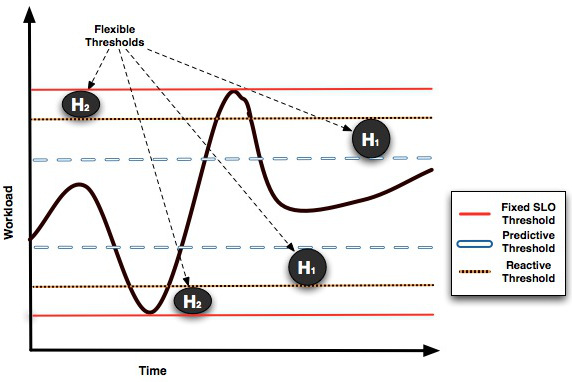
\includegraphics[width=7cm, height=5.3cm]{./images/thresholdGraphic.jpg}
\end{center}
\vspace{-5mm}
\caption{Two-level  thresholds}
\label{flexibleThresholds}
\end{figure}

%\corina{Are the terms ``constant'' and ``temporal'' alteration normally
%used in trend estimation, or are they terms that you defined yourself?
%In the second case I think we should mention something like ``we define constant alteration as...''.  
%And about flash crowds: from what I know, flash crowds last usually longer
%(in the order of hours) and we do want the system to provision extra
%resources in such a case. So if there is a spike of high workload that
%lasts for 10-15 minutes, I don't think we should call it a flash crowd --
%maybe just spike or fluctuation or something like this.}

%In order to take scaling decisiong using the feedback algorithm we now collect application-specific metrics for our measurements, evaluate the %evolution of the application workload avoiding an excessive reactive behavior, and handle threshold values that helps to predict possible SLA violations. 

%In particular, the profiling techniques appears as a solution to tackle this problems of heterogeneity.
\vspace{3mm}

%Anyway, the use of these three mechanisms must follow an order, as illustrated in Algorithm~\ref{history_prov}. Initially, the user has to specify the thresholds %ranges and give a weight to each metric. Next the flexible thresholds are defined based on Amazon recommendations and statistically-chose performance %measures~\footnote{These performance values are obtained from previous executions of the same application using similar hardware configurations.}. Once the %monitoring data is collected from the agents, the decision making process can start. Firstly, these data is analyzed to verify if it exceeds the predictive threshold %ranges (denoted by \emph{pred\_thr}), if so the probability of triggering scaling actions increases proportionally in function of the metric's weight. In order to keep %track of workload variations, this algorithm stores in a queue (denoted by \emph{q}) the most recent system performance values, and analyzed them  to estimate %the workload trend (denoted by \emph{td}).  Finally, to trigger any scaling action, a serie of conditions have to be satisfied: (i) no previous scaling actions have been %taken over the last 15min; (ii) the recent monitoring data have to exceed the predictive and reactive threshold ranges; (iii) the workload trend has to follow a %constant pattern (increasing/decreasing). 


%\subsection{Workload mix-aware provisioning}
\subsection*{Dynamic load balancing weights}

%The heterogeneity of cloud platforms, and therefore, of their VMs affect to the accuracy of the provisioning decisions. VMs with better hardware configuration can sustain higher workload intensities. In addition, the mixture of static/dynamic requests included into the workload of web applications makes more difficult to distribute these requests across multiple backend servers. Most of existing web load-balancer systems provide simple methods which do not consider the workload mix. Hence, methods such as\emph{round-robin} distributes the requests according to the servers with respect of its server weight; and the \emph{least connections} method which distributes requests to the server with the least connections. Unfortunately, these load-distribution methods are not so accurate when having a large diversity in the complexity of the requests. 

%As a solution, the workload mix-aware algorithm proposes to use a dynamic-weight load balancing method in conjunction with the feedback algorithm. By using this dynamic load-balancing mechanism, each backend server has a weight value which is dynamically adjusted based on its monitoring data, and thereby based on its own performance behavior. This mechanism allows to distribute requests across the servers taken into consideration the current workload intensity and the server throughput, which vary depending of its hardware configuration. As illustrated in Algorithm~\ref{mix_prov}, this algorithm assigns the same weight to each backend servers at the beginning of the process, and progressively adjusts their weights  (every $\sim$ 15min) depending on the monitoring data collected from each backend. By doing so, the load-balancing takes into account the complexity of the served requests and inherently the server throughput improving the distribution.

The problem we consider here is the heterogeneity of cloud platforms.
Different virtual machines from the same cloud might have different performance
characteristics, even when their specifications from the cloud vendor are 
the same~\cite{ec2Performance}. This issue can be addressed through various 
load balancing techniques, like assigning weights to the backend servers or 
taking into account the current number of connections that each server 
handles. Furthermore, the performance behavior of the virtual servers may 
also fluctuate, either due to changes in the application's usage 
patterns, or due to changes related to the hosting of the virtual servers 
(e.g., VM migration).

In order to address these issues in ConPaaS we implemented a weighted 
load balancing system in which the weights of the servers are 
periodically re-adjusted automatically, based on the monitoring data.  
This method assigns the same weight to each backend server at the 
beginning of the process. The weights are then periodically
adjusted (in our experiments, every $\sim$ 15min) proportionally 
with the difference among the average response times of the servers 
during this time interval. By adding this technique to the feedback-based
algorithm, we noticed a performance improvement when running the
benchmarks, as discussed in the following.

%%%%%%%%%%%%%%%%%%%%%%%%%%
\begin{comment}
\begin{algorithm}
{\scriptsize
\SetAlgoLined
\SetInd{0mm}{2mm}
\KwData{ Pre-defined metric threshold ranges, \emph{SLO\_threshold}\\
\hspace{9mm} Define the weight of each metric, \emph{w}
}
\KwResult{Scaling decisions}
\BlankLine
Create a queue to store historical workload, \emph{q}\;
Establish flexible thresholds: \emph{pred\_thr} and \emph{reac\_thr}\; 
Initialize load-balancing weights for the backend servers\;
\BlankLine
\While{auto-scaling is ON}{
Collect monitoring data of each metric, \emph{data}\;

\uIf{ avg(data$_i$) $>=$ pred\_thr\_max$_i$}{
	Increment chances of \emph{scaling\_out} using \emph{w$_i$}, \emph{s\_out}\;
}\ElseIf{ avg(data$_i$) $<$ pred\_thr\_min$_i$}{
	Increment chances of \emph{scaling\_back} using $w_i$, \emph{s\_bck}\;
\Else{
Decrease the chances - \emph{s\_bck} or \emph{s\_out}\;
}}
\BlankLine
Add to \emph{q} the most recent workload value\;
Estimate historical workload trends (last $\sim$20min), \emph{td}\;
\hspace{3mm}	- Increasing, \emph{td} = 1 / Decreasing, \emph{td} = 0\;		
\BlankLine
\If{ no recent scaling operation}{
\uIf{ avg(data$_i$) $>=$ reac\_thr\_max$_i$ \textbf{and}  $td$ = 1 \textbf{and} \emph{s\_out} $>=$ \emph{s\_bck}}{
	ADD resources\;
}
\ElseIf{ avg(data$_i$) $<$ reac\_thr\_min$_i$ \textbf{and} \emph{td} = 0 \textbf{and} s\_out $<$ s\_bck }{
	REMOVE resources\;
}
Reset \emph{s\_bck} and\emph{s\_out}\;
}\Else{ Sleep during 5 minutes\;}
\BlankLine
Adjust load-balancing weights based on the workload ($\sim$15min)\;
}
}
\caption{Dynamic load-balancing weights}
\label{mix_prov}
\end{algorithm}
\end{comment}

%%%%%%%%%%%%%%%%%%%%%%%%%%%%%%%%%%

%\fixme{unlike in some synthetic benchmarks, in Wikipedia there are large variations
%in the complexity of the articles; so the PHP processing time is more difficult 
% to predict}

%\begin{figure}
%\begin{center}
%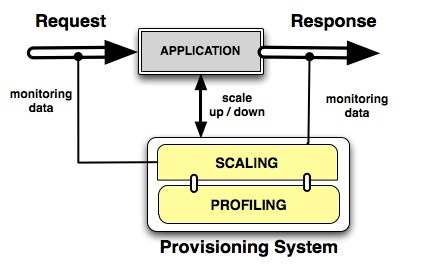
\includegraphics[width=0.4\textwidth, height=4cm]{./images/monitoringSchema.jpg}
%\end{center}
%\label{model}
%\caption{Profiling Resource Provisioning}
%\end{figure}


\section*{Evaluation \label{experiments}}

To compare the provisioning algorithms described above, we ran experiments
on two infrastructures: a homogeneous one (the DAS-4, a multi-cluster system
hosted by universities in The Netherlands~\cite{das4}) and a heterogeneous
one (the Amazon EC2 cloud~\cite{amazonEC2}). The goal of our experiments
was to compare the algorithms by how well they fulfill the SLOs and by
the amount of resources they allocate.

%In this section we conducted our experiments on a heterogeneous infrastructure like Amazon EC2~\cite{amazonEC2}, and on a homogeneous infrastructure like DAS-4 (the Distributed ASCI Supercomputer 4)~\cite{das4}. In our experiment campaign, we compared the degree of SLO enforcement and resource consumption for each provisioning algorithm implemented in ConPaaS. 

%DAS-4 is the Dutch Computational Infrastructure, a six-cluster wide-area distributed system designed with research purposes

\textbf{Testbed configuration:}  As a representative scenario, we deployed the MediaWiki application using ConPaaS on both infrastructures, and we ran the Wikibench tools with a 10\% sample of a real Wikipedia access trace for 24hours. 
%Consequently, our goal is to evaluate the behavior of the provisioning algorithms, when scaling out and back the number of VMs hosting PhP servers to guarantee several performance requirements, referred to as SLO.  Accordingly, some assumptions were made:
We configured the experiments as follows: 

\begin{itemize}
%\item  Response times from static requests were not analyzed due to its lightweight nature. 

\item The monitoring data was collected over a reporting period of 5 minutes.

\item We fixed a SLO of 700 milliseconds at the service's side (denoted by a red Line on Figures~\ref{naiveDas4},\ref{historyDas4},\ref{naiveEC2},\ref{historyEC2}).


\item The dynamic load-balancing weights provisioning technique was only evaluated on the heterogeneous platform, Amazon EC2. This algorithm brings improvements to the feedback algorithm only in environments where VMs may have different hardware configurations. 

\item The algorithms used the same statistically-chosen performance threshold ranges. 

%\item A minimum interval of 15 minutes has been established between scaling actions to avoid excessive oscillations. 
\end{itemize}


%To provide the Wikipedia services, an initial configuration was composed of 4 VMs, and 1 VM to host the Wikibench tools. The 4 VMs include a PhP service manager VM, a PhP agent VM, a web server and a http-proxy agent VM (both in the same VM), and finally a MySQL agent VM to store the English Wikipedia data, as explained in Section~\ref{wikipedia}.

\subsection*{Homogeneous Infrastructure}

Our experiments on DAS-4 rely on OpenNebula as IaaS~\cite{sotomayor_virtual_2009}. To deploy the Wikipedia services, we used small instances for the PHP service (manager and agents) and a medium instance for the MySQL service (agent). In DAS-4, OpenNebula's small instances are VMs equipped with 1 CPU of 2Ghz, and 1GiB of memory, while medium instances are equipped with 4 CPU's of 2Ghz, and 4GiB of memory.

\paragraph{SLO enforcement.}
Figure~\ref{naiveDas4} and Figure~\ref{historyDas4} represent the degree of SLO fulfillment of the trigger-based and feedback algorithms, indicating the average of response times obtained during the execution of the Wikipedia workload trace. The results from Figure~\ref{naiveDas4} show that the trigger-based provisioning algorithm provokes an important amount of SLO violations at certain moments in time, due to its excessively reactive behavior. As we mentioned, this algorithm fails easily during traffic spikes, as it adds or removes VMs without evaluating the workload trend. The feedback algorithm, as shown on Figure~\ref{historyDas4}, handles the traffic spikes better and can achieve fewer SLO violations; specifically, there were 31.72\% less SLO violations in comparison with the trigger-based algorithm. 


\begin{figure}

\begin{center}
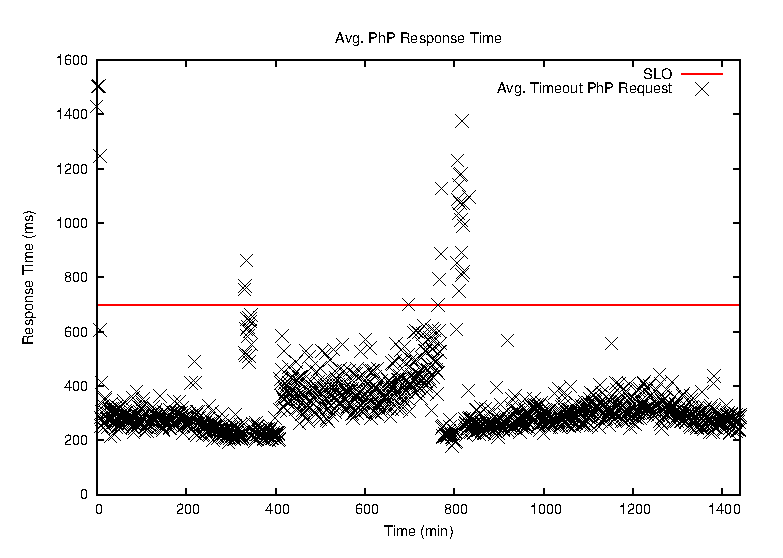
\includegraphics[width=0.49\textwidth, height=6cm]{./images/homogeneous/avgTimeout_PhP_trigger}
\end{center}
\vspace{-5mm}
\caption{Response time on DAS4 -- Trigger-based.}
\label{naiveDas4}
\end{figure}

\paragraph{Resource consumption.}

To better understand the behavior of both algorithms, we shall also focus on the resource consumption illustrated on Figure~\ref{resComDas4}. The excessively reactive behavior of the trigger-based algorithm can be noticed in the time intervals around \emph{t=350min} and \emph{t=820min}, where two scaling operations under-provision the system during a short period of time. These provisioning decisions provoked the SLO violations that are visible in Figure~\ref{naiveDas4}in the same intervals of time. Besides affecting the system's stability, such short fluctuations in the number of provisioned resource also raise the cost of hosting the application since more VM instantiations will be triggered. When using the feedback algorithm, the system makes provisioning decisions by analyzing the workload's trend. Scaling actions are only triggered when having \emph{constant} alterations in the workload, thereby providing a more efficient resource usage. We can see that the provisioning decisions made by the feedback algorithm on Figure~\ref{resComDas4} match well with the workload alterations depicted on Figure~\ref{workload}.

\begin{figure}
\begin{center}
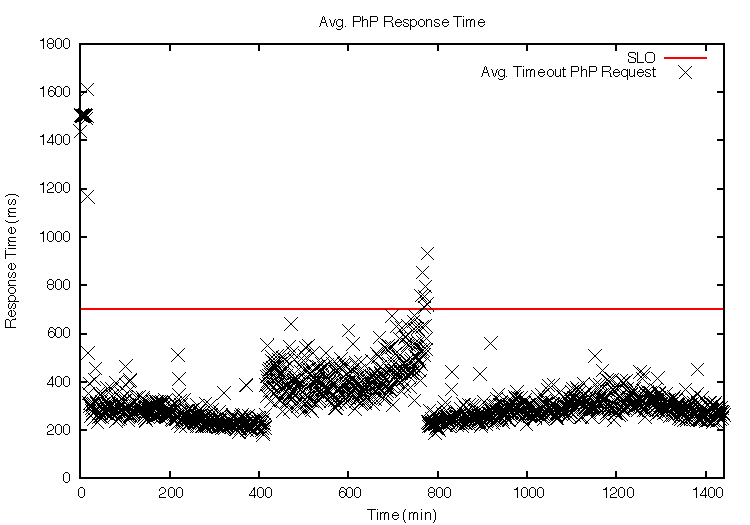
\includegraphics[width=0.49\textwidth, height=6cm]{./images/homogeneous/avgTimeout_PhP_feedback}
\end{center}
\vspace{-5mm}
\caption{Response time on DAS4 -- Feedback.}
\label{historyDas4}
\end{figure}

\begin{figure}
\begin{center}
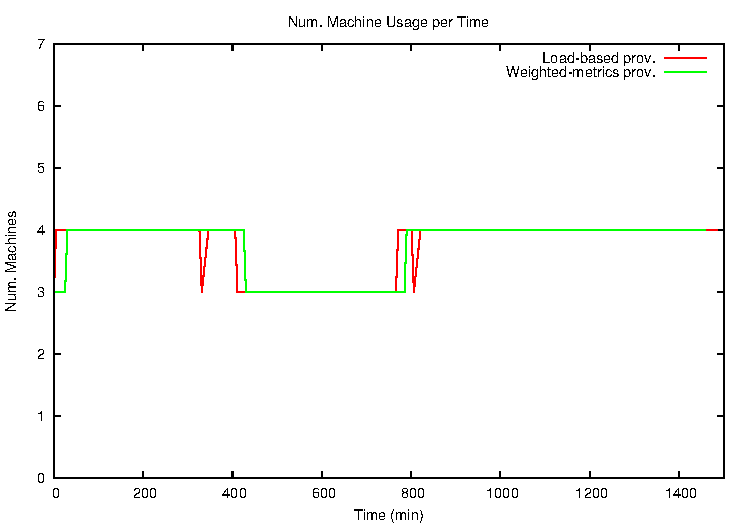
\includegraphics[width=0.49\textwidth, height=5cm]{./images/homogeneous/numMachinesComp}
\end{center}
\vspace{-5mm}
\caption{Resource consumption on DAS4.}
\label{resComDas4}
\end{figure}

\paragraph{Discussion.}

%Using the trigger-based provisioning algorithm, the system performance fluctuates greatly following a pattern similar to the web traffic, that increases the amount of SLO violations. The reactive behavior of this algorithm triggers scaling actions that affect to the system performance instead of improving it, and as a consequence, it is also wasteful in terms of resource consumption. Unlike feedback algorithm offers an efficient resource usage and a constant performance behavior while meeting the application's SLO. 

%Therefore this algorithm finds the trade-off between accuracy and cost savings.

%Both algorithms are best-effort regarding the SLO fulfillment, and thereby temporal alterations of the workload (with a short duration of 5min approx.) cannot be handled. The heterogeneity of the PhP-requests including images and requiring multiple Db queries, as well as the startup time of VMs (2-5min), are in part responsible of these SLO violations. 

Both algorithms are best-effort regarding the SLO fulfillment, and thus they do not handle well short alterations of the workload (with duration in the range of minutes). The heterogeneity of the PHP requests, as well as the startup time of VMs (2-5min), are in part responsible of these SLO violations.

%It avoid to under-provisioning in two occasions  while decreases the number of SLA violation. However, the naive alg. is vulnerable to temporal bursty workload variations (10 min), an increment of SLA violated is caused by under-provisioning operations in conjunction with workload variations. 



\subsection*{Heterogeneous Infrastructure}

Our experiments on EC2 used small instances for the PHP service (manager and agents) and  a medium instance for the MySQL service (agent). EC2 small instance are equipped with 1 EC2 CPU, and 1.7GiB of memory, while medium instances are equipped with 2 EC2 CPU's, and 3.75GiB of memory.

%In the following, we analyze the behavior of our algorithms when making provisioning decisions on a heterogeneous infrastructure.

\paragraph{SLO enforcement.}
Figure~\ref{naiveEC2}, Figure~\ref{historyEC2} and Figure~\ref{historyWeightEC2} show the system performance of the trigger-based, feedback and dynamic load-balancing weights algorithms, respectively. As depicted on Figure~\ref{naiveEC2}, the performance of the trigger-based algorithm is even more unstable than in the case of the homogeneous infrastructure. Two of the three peaks in response time, at \emph{t=300min} and \emph{t=820min}, can be explained by the variations in the Wikipedia workload shown in Figure~\ref{workload}. However, there is a third peak between \emph{t=400min} and \emph{t=500min} that corresponds to an interval of time in which the workload trace shows a significant drop in the request volumes. During this period of time, the algorithm attempts to scale down the system but the new lower number of resources cannot handle the load, and the system is scaled up again. As this algorithm does not keep any history information, after a short time it attempts again to scale down the system, with the same result; thus, some oscillations occur in the number of allocated resurces, causing also SLO violations.   

Figure~\ref{historyEC2} and Figure~\ref{historyWeightEC2} show that the
feedback and dynamic load-balancing algorithm reduce the number of SLO 
violations and provide a more stable performance pattern. Specifically,
with the feedback algorithm  we obtained 41.3\% less SLO violations than
with the trigger-based algorithm, while the dynamic load balancing algorithm
had 47.6\% less violations than the trigger-based one.

%On the other hand, Figure~\ref{historyEC2} and Figure~\ref{historyWeightEC2} show as the feedback and dynamic load-balancing weight algorithm behave similarly. Even though both algorithms are best-effort, there is an important reduction in the number of SLO violations during the trace execution. In particular, the feedback algorithm reduces the SLO violations in a  41.3\%, while the dynamic load-balancing weights algorithm does it in a 47.6\%. Like on DAS-4, the feedback algorithm presents a stable performance pattern without having sudden and bursty workload alterations. Besides, as shown on Figure~\ref{historyWeightEC2}, the dynamic load-balancing weights algorithm algorithm has a similar behavior to the feedback algorithm in terms of system performance, however. This algorithm improves the SLO enforcement in a 6.3\% in comparison with feedback at the client's side. 

%Therefore we demonstrate how the use of workload-mix and flexible load-balancing techniques, although intrusive, do not cause time delays or excessive throughput alterations. 



\begin{figure}
\begin{center}
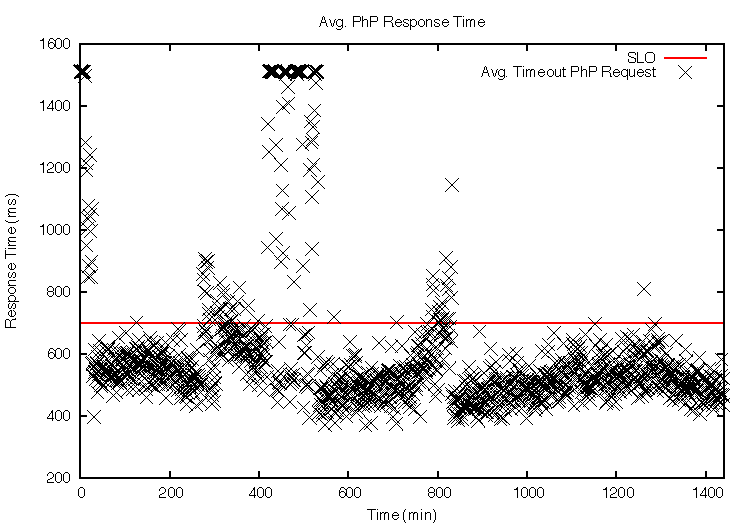
\includegraphics[width=0.49\textwidth, height=6cm]{./images/heterogeneous/avgTimeout_PhP_trigger}
\end{center}
\vspace{-5mm}
\caption{Response time on EC2 -- Trigger-based.}
\label{naiveEC2}
\end{figure}


\begin{figure}
\begin{center}
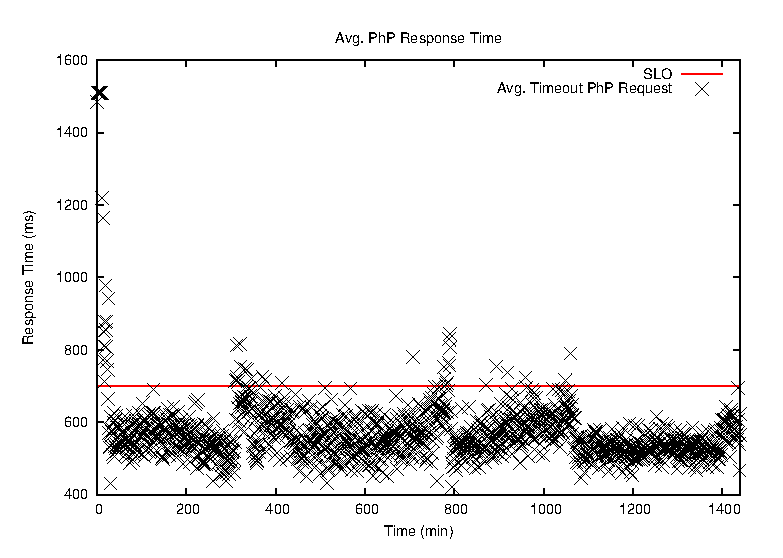
\includegraphics[width=0.49\textwidth, height=6cm]{./images/heterogeneous/avgTimeout_PhP_feedback}
\end{center}
\vspace{-5mm}
\caption{Response time on EC2-- Feedback.}
\label{historyEC2}
\end{figure}

\begin{figure}
\begin{center}
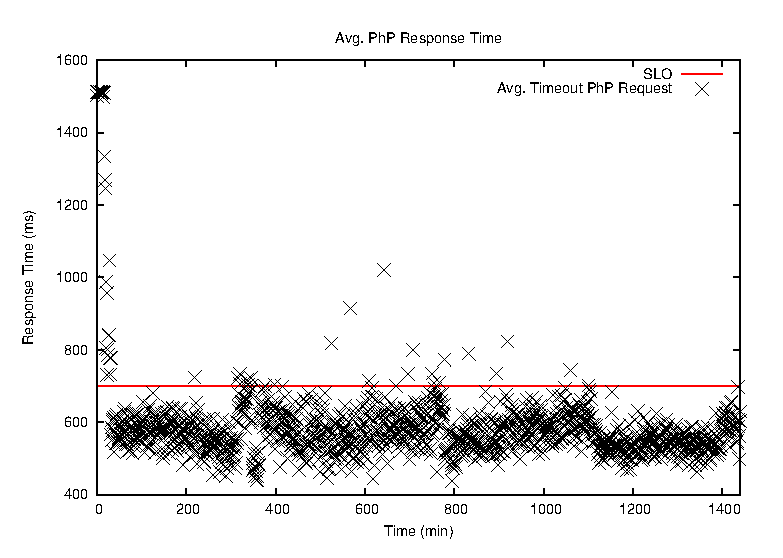
\includegraphics[width=0.49\textwidth, height=6cm]{./images/heterogeneous/avgTimeout_PhP_DLBweights}
\end{center}
\vspace{-5mm}
\caption{Response time on EC2-- Load-balancing Weights.}
\label{historyWeightEC2}
\end{figure}

\paragraph{Resource consumption.}
As explained above, the trigger-based algorithm sometimes initiates
series of scaling back quickly followed by scaling out operations, 
due to the fact that it does not use any history information that could
prevent these oscillations. This can be seen on Figure~\ref{resEC2},
in the time interval between \emph{t=400min} and \emph{t=500min}.
The feedback and dynamic load balancing algortithms have similar
and more stable patterns of resource consumption, which show the
benefits of using trend estimations and two-level threshold ranges.

%The resource usage on EC2 presents important changes, as shown on Figure~\ref{resEC2}. When using the trigger-based provisioning, the fluctuations in the system performance are explained as a result of a high frequency of scaling operations. In concrete, the fluctuations caused at the interval of time between \emph{t=400min} and \emph{t=500min} (see on Figure~\ref{naiveEC2}), match with the provisioning decisions made during the same interval of time on Figure~\ref{resEC2}. If we now pay attention to the feedback, and dynamic load-balancing weights algorithms, their resource consumptions are identical along the execution. Indeed, both algorithms decided to scale out the system during the interval of time comprised between \emph{t=1050min} and \emph{t=1400min}, to prevent future SLO violations that occurred when looking at the trigger-based algorithm on Figure~\ref{naiveEC2}. In particular, this situation demonstrates the benefits of using two-level threshold ranges to provide a predictive provisioning mechanism, thus improving the user experience.


\begin{figure}
\begin{center}
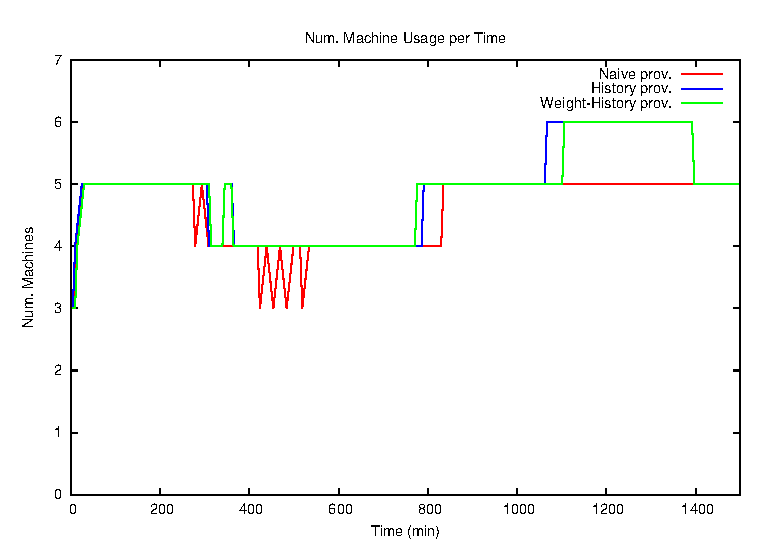
\includegraphics[width=0.49\textwidth, height=5cm]{./images/heterogeneous/numMachinesCompEC2}
\end{center}
\vspace{-5mm}
\caption{Resource consumption on EC2.}
\label{resEC2}
\end{figure}


\paragraph{Discussion.}
In order to have a better estimation of the algorithms' performance, we 
ran the experiments on Amazon EC2 a second time. The results of the two 
runs are summarized in Table~\ref{summaryEC2}, where we show the percentage
of SLO violations from the total number of requests, the number of
provisioning decisions (scaling out or back) taken by the algorithms
and an estimation of the cost of runnning the VMs in Amazon EC2.

Firstly, we noticed performance differences between the two runs of the
experiments, which are due to the fact that each experiment was run on
a different set of VMs from EC2. The trigger-based alogrithm in particular
is quite sensitive to small changes in the VM characteristics: since it
uses only one set of thresholds and no information about the workload
trend, it easily becomes unstable and may behave differently from one
run to another.

Secondly, both runs show significant differences between the trigger-based
algorithm on one hand, and the feedback and dynamic load balancing on
the other hand. The results show that using a few euristics as in the last
two algorithms can help in improving the performance and stability
of the system. We did not obtain however significant differences
between the feedback and the dynamic load balancing algorithm. The last
algorithm uses the additional technique of dynamically adjusting the
load balancing weights, but the the VMs participating in the experiments 
had relatively similar performance and adjusting their weights only
made a small difference. On other infrastructures that are more heterogeneous
than Amazon EC2, the dynamic load balancing technique may bring
a greater performance improvement.  

We also note that the cost of the trigger-based algorithm is slightly
lower than the cost of the other two algorithms. This algorithm
attempts more often to scale down the system, which explain the lower cost;
but on the other hand, this leads to more SLO violations and more
instability: many VM instances created and then shut down very soon. 

%The experiments on EC2 leads to several conclusions. The use of the trigger-based algorithm shows again how aggressive provisioning increases the resource consumption and the chances of degraded application performance due to frequents scaling actions. These actions are triggered as an effect associated to the traffic and heterogeneity of the requests, when handling bursty workload conditions. On the other hand, the feedback and dynamic load-balancing algorithms constitute two robust provisioning models that offer an efficient resource consumption and keep stable the application performance during the trace execution. 

%Furthermore, the use of a dynamic load-balancing algorithm provided a more efficient distribution of the request-mix across servers, that reduced the SLO violations in a 6.3\%. Hence, the main objective behind of this algorithm is to tackle the degradations caused by the workload heterogeneity.


%{\scriptsize
%\begin{table}
%\begin{center}
  %  \begin{tabular}{ | l | c | c |}
  %  \hline
  % \textbf{Algorithm}   & \textbf{DAS4} & \textbf{EC2}   \\ \hline
  %  Trigger-based & 3808 &  30357    \\ \hline
  %  Feedback &	2601 & 17856 \\ \hline
 %   Dynamic load-balancing   & -- & 15931\\ \hline
%\textbf{Num. of requests}  & 384501 & 438430  \\ \hline
  %  \hline
	
 %   \end{tabular}
%\end{center}
%\caption{SLO violations at the client's side (1500ms).}
%\end{table}
%}

\begin{table*}\label{summaryEC2}
  {\scriptsize 
\begin{center}
    \begin{tabular}{  | c | c | c | c | c | c | c | c | c |}
    \hline
    \multicolumn{3}{|c|}{ \textbf{Trigger}  } & \multicolumn{3}{|c|}{ \textbf{Feedback} }&  \multicolumn{3}{c|}{ \textbf{Load-balancing}  }   \\ \hline 
 \textbf{SLO Violations}& \textbf{Decisions} & \textbf{Cost} & \textbf{SLO Violations} & \textbf{Decisions} & \textbf{Cost} & \textbf{SLO Violations} & \textbf{Decisions} & \textbf{Cost} \\ \hline
  6.92\% & 14 & 7.5 &  4.07\%  & 8 & 7.7 &  3.63\% & 8 & 7.7  \\ \hline
  13.7 \% & 28 & 7.86 &  3.96\%  & 8 & 8.4 &  4.07\% & 8 & 8.32  \\ \hline
 \end{tabular}
\end{center}
\vspace{-5mm}
\caption{Analysis of results on EC2}
}
\end{table*}



%\subsection*{Discussion}

As a conclusion, we found from our experiments that a simple trigger-based
provisioning mechanism does not handle workload variation well and
in some situations causes instability, by changing the number of
provisioned VMs often in short time intervals. This behaviour has a 
negative effect on the application's response time, leading to violations
of the SLO.

By using a few techniques that are relatively easy to implement (like
estimating the workload's trend for the last 30 minutes and using
two levels of thresholds for the provisioning metrics) we showed that
we can significantly reduce the number of SLO violations and
obtain more stability. Although there is still room for improvement
in our techniques, from the experimental results we can draw the
conclusion that implementing provisioning mechanisms that go
beyond simple triggers is effective and should be considered
when hosting a cloud application.

%Generally, the result of our measurements show how the behavioral performance pattern and the resource consumption vary depending on the infrastructures on which we ran our experiments. Different hardware configurations such as those provided by DAS-4 and EC2, offer two distinct scenarios to validate our provisioning algorithms.  In these experiments, we demonstrate how trigger-based provisioning mechanisms can affect the system performance instead of improving it, as well as are wasteful in terms of resource usage. Furthermore, we show how a dynamic load-balancing technique, although intrusive, can be included and used without producing performance alterations. In fact, this technique slightly reduced the number of SLO violations in comparison with the results obtained using feedback algorithm. Finally, we also present the benefits by using feedback and dynamic load-balancing weights provisioning algorithms which aims to find the trade-off between the accuracy and cost savings. 

%However, there is room for improvement using the dynamic load-balancing weights algorithm, as some  workload alterations could not be handled during the trace execution.

%the flexible threshold ranges were pre-defined before execution for all VMs. These threshold values might be %changed depending the type of instance to be provisioned. Therefore, we believe that offline profiling techniques %may be used to define these values depending of the type of instance, thus improving the effectiveness of our %predictions.

%Today's resource provisioning systems define SLO's based on desirable threshold values for an application (CPU %$<$ 70\% and resp. time $<$= 700ms). However, these threshold values change depending the type of instance %to be provisioned (\emph{i.e.,} small instances 200 $<$ resp. time $<$ 500, while medium instances 200 $<$ %response time $<$ 600). In order to improve the accuracy of these algorithms, we consider that provisioning %decisions have to take into account two threshold ranges: (i) desirable threshold values for the whole application; %(ii) specific threshold values for each machine. Thus, to determine these machine-specific threshold values, offline %profiling techniques have to train during a period of time 





\section*{Related studies \label{studies}}


There is a wide literature on issues related to dynamic resource provisioning for cloud web applications. Different approaches present solutions based on queuing models~\cite{urgaonkar_agile_2008}, feedback loops techniques~\cite{gong_gray-box_2010}, mathematical models~\cite{muppala_regression-based_2012} or even approaches using neural networks techniques~\cite{islam_empirical_2012}. However, most of these models require a deep understanding in mathematics or machine learning techniques which are not easily interpreted by non specialists. Besides the traffic in web applications is shaped by a combination of different factors such as diurnal and seasonal cycles, sociological and psychological, that follows an irregular pattern. It makes extremely challenging the design and development of realistic and accurate dynamic provisioning mechanisms. 

These well-known drawbacks force to IaaS like Amazon EC2 and Windows Azure~\cite{azure}, or PaaS like RightScale~\cite{right-scale} and OpenShift~\cite{openshift},  to design simple threshold rule-based auto-scaling systems, instead of relying on approaches from academic research. Unfortunately, these scaling systems are naive, wasteful in terms of resource consumption and cost savings, and an easy target for flash crowds.

% Workloads follow irregular patterns including “flash crowds".

% It is slow to workload changes and not effective at handling complex load
%patterns experienced in practice. Besides, over peak load reactive dynamic provisioning typically does no more than overprovisioning over one computing resource, while %the provisioning over other resources including storage and networking is not explicitly addressed or optimized.

In the following, we present some of the most relevant and realistic academic approaches that proposed dynamic resource provisioning mechanisms for multi-tier applications. 

%As we mentioned, offline and online profiling are promising techniques when handling unpredictable and temporal burstly workloads in web applications.  

In ~\cite{urgaonkar_agile_2008, urgaonkar_cataclysm:_2008}, the authors designed and implemented a predictive and reactive provisioning mechanism. They used a queuing model  G/G/1 to decide the server pool size to be provisioned, and an admission control mechanism to face extreme workload variations. Offline prolifing techniques were employed to gather information about the resource requirements of the incoming requests for each tier, and thereby to selectively admit/reject requests for the lightweight files.  An evaluation using real-traces on a homogeneous infrastructures shows the benefits of this approach when handling flash crowds. Unfortunately, its admission control mechanism incurs into sporadic SLA violations ( if the server utilization exceed a pre-defined threshold) reducing the QoS of the service, and therefore affecting user experience. Similarly to the previous work, \cite{wang_appraise:_2009} extended queuing models and transaction mix models to design a predictive and reactive provisioning system. To model the application performance, they integrated proactive control and feedback control methods that dynamically adjusted the CPU capacity allocated to servers. This work only considered SLA constraints at the hardware level, while others constraints at the application level such as response time and request rate were not taken into consideration. Besides, an evaluation of CPU variations on a homogeneous infrastructure, when processing traces from a non real-world application, lack arguments to valid its approach.

%control and dynamic provisioning components in addition to the load balancing algorithm. It applies admission control to make sure flash crowd requests
%will not overload the provisioned server pool by dropping requests, and uses queuing-model based dynamic provisioning technology.

Regarding the management of flash crowds~\cite{zhang_resilient_2009}, a proactive application workload manager was designed to separate the user requests between two groups of servers:  one  named  'base workload'  referred to the smaller and smoother variations in the workload; and the other 'tresspassing' referred to the temporal burstly workloads caused by flash crowds. To do this, the authors attempt to divide the data items into popular and less popular, and place them in the right group of servers. Even tough a realistic evaluation was conducted on Amazon EC2 utilizing real traces (Yahoo video streaming), authors do not explain in details how the dynamic resource provisioning is done. Recently, in  \cite{kaviani_profiling-as--service:_2011}, online profiling techniques have been utilized for managing the tradeofff between performance overload, and cost savings for dynamic resource provisioning. The authors replicate at runtime a regular server hosting an application, with a new server with profiling instrumentation. Their experimental results show how profiling techniques can be included in a resource provisioning system, without causing important response time delays or throughput alterations in comparison with non-profiling provisioning. As we mentioned in Section~\ref{}, profiling techniques can report more benefits than  performance degradations or expenses.





%\section*{Conclusion \label{conclu}}
% Magazine articles have no section called "Conclusion"
\label{sec:conclusion}



Nowadays cloud infrastructures offer a plethora of distinct hardware configurations for rent and price, we argued that autoscaling systems can use this diversity to better fulfill the SLA requirements without dramatically raising the operational cost. This has special importance for enterprises where a decrease in the user base led to a reduction in revenue, or for cloud providers where penalties paid due to SLO violations have a revenue impact. We proposed a novel autoscaling approach for cloud applications that provisions the most appropriate hardware configuration according to the customer requirements. This system benefits from cloud heterogeneity and online profiling techniques to find a scaling plan adapted to the QoS and current workload requirements. By considering factors such as SLO fulfillment or infrastructure cost, our system minimizes the performance degradations even under large and temporal workload variations. We implemented an autoscaling system that has been successfully deployed in multiple clouds. We evaluated our system in a realistic scenario showing the benefits by selecting a configuration that mitigates the performance degradations even under bursty workload. Nevertheless, these benefits could also be observed along the whole execution of a workload trace. In the future we plan to extend our system by supporting a bigger number of hardware configurations and by optimizing 
the dynamic load balancing mechanism. Similarly, we want to further study the financial impact of combining different hardware configurations.


% integrating a neural network forecasting model
% support for more types of instances.


%It is necessary to highlight the impotance of autoscaling systems that exploits the heterogeneity of the cloud infrastructures when provisioning applications.

%cheapest configuration doesn't have to be efficient. Tradittional system scale out and back using small instances.






\section*{Acknowledgments}

This work is partially funded by the FP7 Programme of the European
Commission in the context of the Contrail project under Grant
Agreement FP7-ICT-257438.



\bibliographystyle{plain}
\bibliography{paper}

\end{document}
